\section{Results} \label{results} 
In order to evaluate the performance of the method described in Section \ref{approach}, we need to compare the predicted network to the real network that generated the data. In real biological applications this procedure is usually not possible, due to the fact that the real network is, in fact, unknown. 
In the specific case described thus far, we take advantage of synthetic data that make such a performance evaluation practical. 

Since our algorithm is designed to analyse gene expression profiles, we generate synthetic microarray data with the Gene Net Weaver software package (GNW) (\citealp{gnw1}). The aim of GNW is to generate in-silico networks extracting modules from biological networks. These networks are simulated to produce gene expression data (steady states or time series) (\citealp{gnw2}). The aforementioned framework can be used to evaluate the performance of our inference method by comparing the predicted network with the golden standard network that generated the dataset. 

We perform the approach described above on synthetic microarray data generated from simulated networks of 50 and 200 nodes. The parameters used in our experiments are summarised in Table \ref{params}.

\begin{table}[htdp] 
%\begin{center}
\begin{tabular}{| l | l |} 
\hline
\textbf{cross-validation} & 3-fold on 10\% genes \\  \hline
\textbf{best} & 80\% genes\\  \hline
\textbf{fanout} & 1 \\ 
\textbf{B} & 0-500 \\ \hline
\end{tabular}
%\end{center}
\caption{Parameters of LABnet for both 50-node and 200-node networks}\label{params}
\end{table}  

\begin{figure*} 
\noindent\begin{minipage}{.5\textwidth}
\centering
  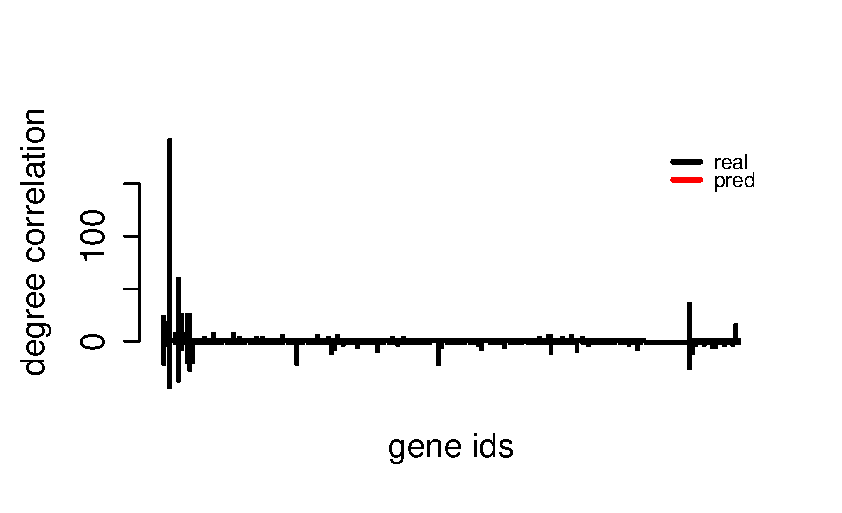
\includegraphics[width=1\linewidth]{degree_barplot.eps}
  \captionof{figure}{Degree correlation across real and predicted nodes}
  \label{fig:degree}
\end{minipage}
\noindent\begin{minipage}{.5\textwidth}
  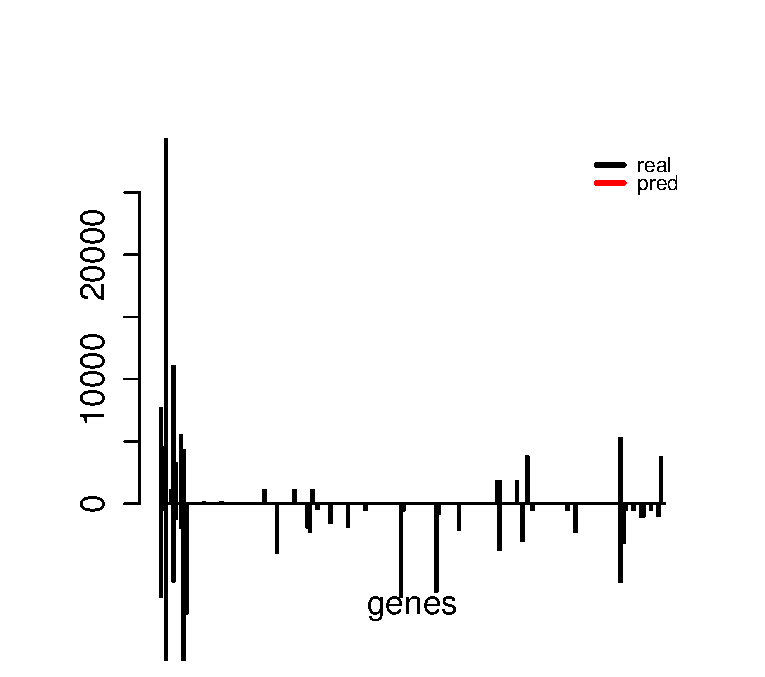
\includegraphics[width=1\linewidth]{between_barplot.eps}
  \captionof{figure}{Betweenness correlation across real and predicted nodes}
  \label{fig:between}
\end{minipage}
\end{figure*}


A set of networks has been inferred with an increasing number of permutations. One important characteristic that arises from our experiments consists in the fact that by increasing the number of permutations, the connectivity of the network is increased proportionally (Figure \ref{fig:pred_fp}). Within the same figure it is shown that the number of false positives is limited regardless the number of predicted edges and permutations.   
We measure the connectivity of the network by counting the number of the predicted edges. 

In Figure \ref{fig:fpr_perm}, the false positive rate, usually referred to as accuracy, is not affected by the number of permutations but by the number of predicted edges which increases accordingly (as shown in Figure \ref{fig:pred_fn}). 

Moreover, by increasing the number of permutations the false negatives, or missed edges, tend to decrease (\ref{fig:fpr_perm}). Since higher connected networks are usually affected by an increasing number of false negatives, we consider the method described above a promising approach with potential benefits to the analysis of large genetic networks. 

We also found that the true positive rate follows the same trend of the number of permutations (Figure \ref{fig:tp_mcc}). Within the same figure the Matthew Correlation Coefficient (MCC) is also reported. The MCC is a correlation coefficient between the observed and the predicted classification (presence or absence of edge) and takes into account both true and false negatives of the overall predicted network. More specifically, the MCC takes into account the number of true negatives of the predicted network within the normalisation factor. For sparse biological networks the number of true negatives is usually high. In an extreme cases of an empty predicted network, the number of true negatives would positively impact the overall performance. It comes without saying that such a metric would be too optimistic. 

The MCC, as introduced in \citealp{Matthews1975}, is calculated as 

\begin{equation}
MCC = \frac{(TP \times TN) - (FP \times FN)}{\sqrt{\splitfrac{(TP+FP)\times(TP+FN)}{
\times(TN+FP)\times(TN+FN)} }}
\label{eq:mcc}
\end{equation}

In order to compare the predicted network to the golden standard using a measure that takes into account the global structures of the graphs, two global measures have been provided, such as the degree correlation $DC$ and the betweenness correlation $BC$.
 
$DC$ is the correlation between the vector of the degrees of all genes in the real network and those of the predicted network. It is calculated as 

\begin{equation}
DC = cor(\bar{d}_{gold}, \bar{d}_{pred})
\label{eq:degree}
\end{equation}

where $d$ is the $i$-dimensional vector containing the degree of each gene. 

Similarly, the betweenness correlation $BC$ is the correlation between the same two vectors where the degree has been replaced by the betweenness centrality measure.

$BC$ is calculated as 

\begin{equation}
BC = cor(\bar{b}_{gold}, \bar{b}_{pred}) 
\label{eq:betweenness}
\end{equation}


where $b=b(i)=\sum_{q \ne i \ne r} \frac{\sigma_{qr}(i) } {\sigma_{qr} } , \forall i$, $\sigma_{qr}$ is the total number of shortest paths from node $q$ to node $r$ and $\sigma_{qr}(i)$ is the number of shortest paths from $q$ to $r$ that pass through gene $i$.


Betweenness centrality is, in our opinion, more helpful than simple connectivity. This measure is a direct indicator of how connected the node is and its importance with respect to the global network topology. 

As it can be seen in Figure \ref{fig:degree} and Figure \ref{fig:between} there is a strong degree correlation (0.83) and betweenness correlation (0.86) between the nodes of the predicted and real networks. The two measures and the aforementioned strong correlations support the evidence that the topology of the real network is conserved within the predicted network, following the same power law degree distribution of the original network that generated the data. 
Due to the fact that GNW generates network from real life templates, we expect  similar results in real biological data.


\begin{figure*} 
\noindent\begin{minipage}{.55\textwidth}
  \centering
  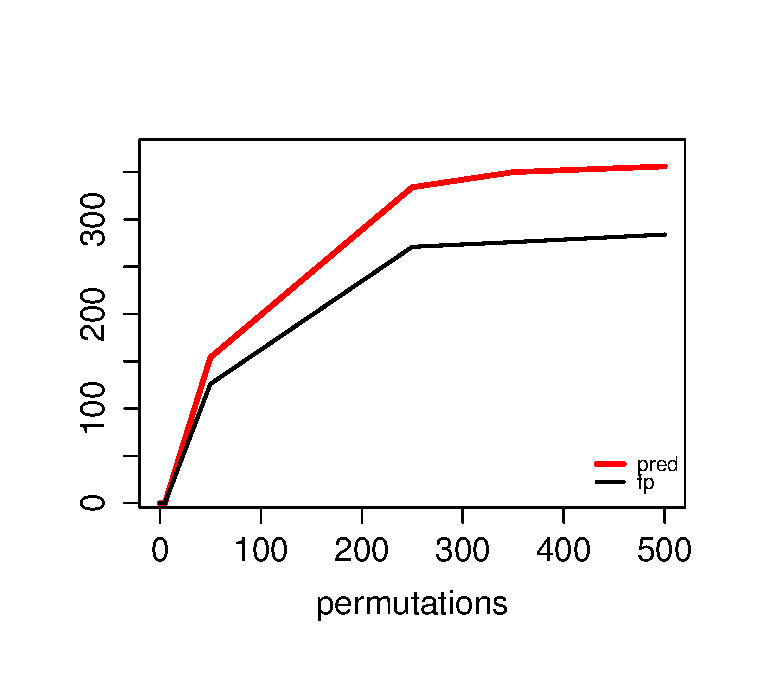
\includegraphics[width=.8\linewidth]{pred_fp.eps}
  \caption{Number of predicted edges and false positives vs. \\ number of permutations}
  \label{fig:pred_fp}
\end{minipage}%
\noindent\begin{minipage}{.55\textwidth}
  \centering
  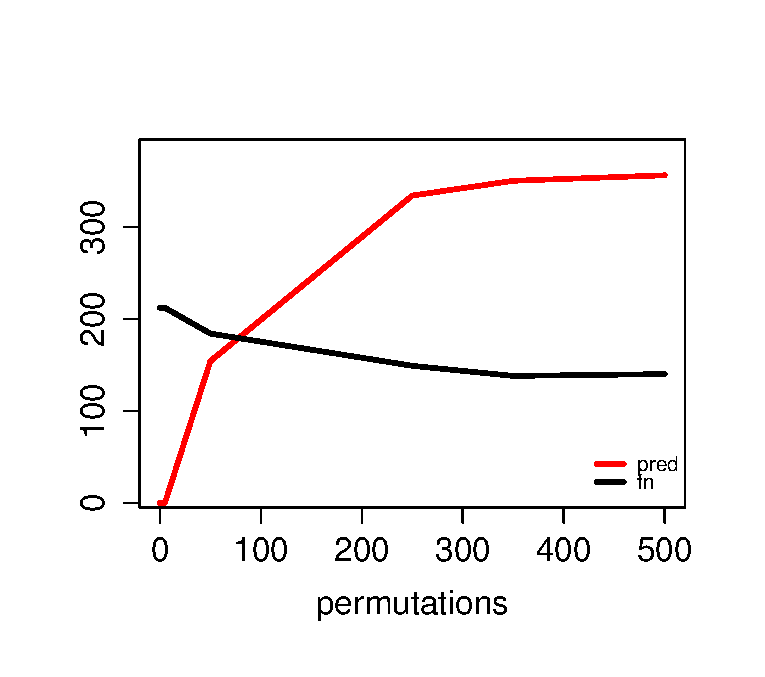
\includegraphics[width=.8\linewidth]{pred_fn.eps}
  \caption{Number of predicted edges and false negatives vs. \\ number of permutations}
  \label{fig:pred_fn}
\end{minipage}
\begin{minipage}{.55\textwidth}
  \centering
  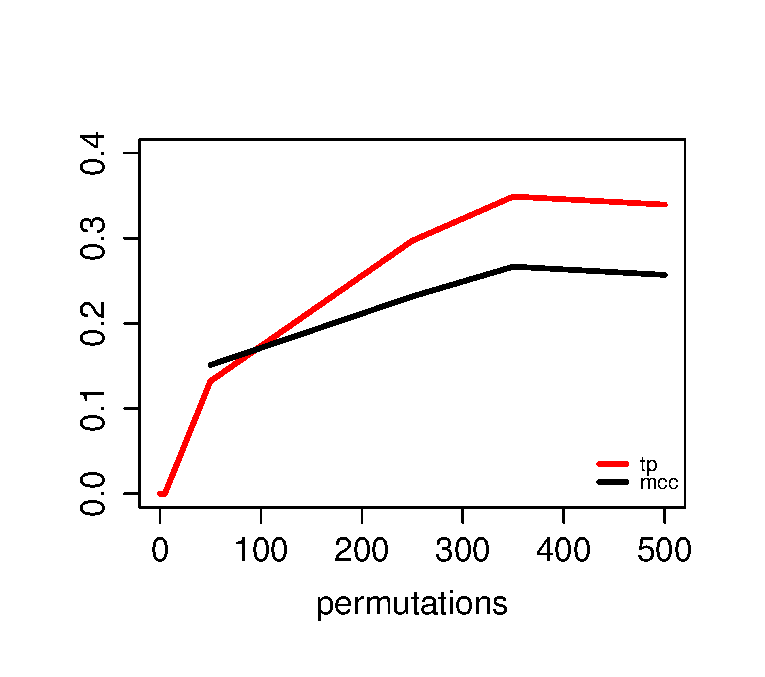
\includegraphics[width=.8\linewidth]{tp_mcc.eps}
  \caption{True positives and Matthew Correlation Coefficient vs. \\ number of permutations}
  \label{fig:tp_mcc}
\end{minipage}%
\begin{minipage}{.55\textwidth}
  \centering
  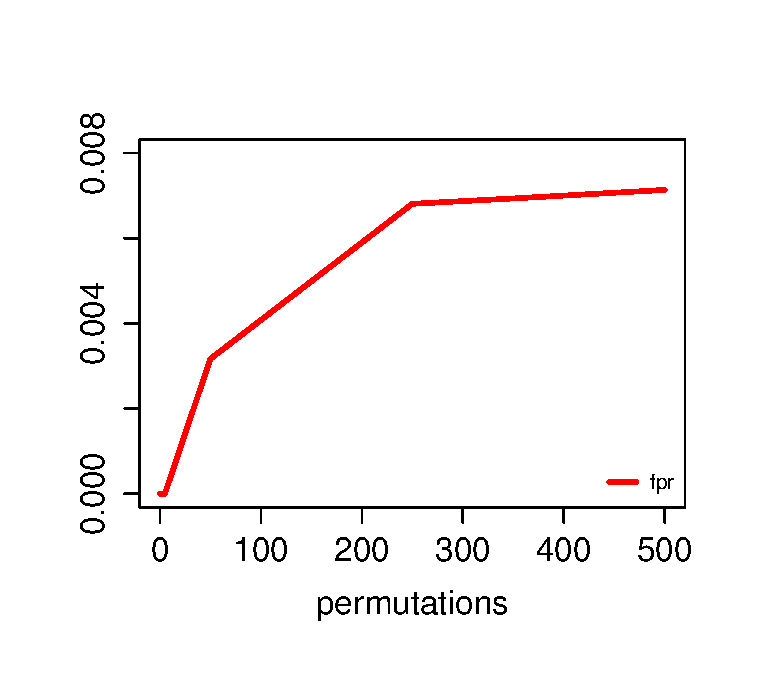
\includegraphics[width=.8\linewidth]{fpr.eps}
  \captionof{figure}{False positive rate vs. number of permutations}
  \label{fig:fpr_perm}
\end{minipage}
\label{fig:global}
\end{figure*}


